\documentclass[11pt]{article}
\usepackage[textwidth=18.0cm, textheight=23.0cm, top=2.0cm]{geometry}
\usepackage{pst-all}
\usepackage{amssymb}
\usepackage{tikz}
\usepackage{underscore}\begin{document}
\pagestyle{empty}


ClassName: \underline{\textbf{Class_03.2bp-25}}
\par
BinSize: \underline{\textbf{40 × 40}}
\par
ReduceSize: \underline{\textbf{40 × 40}}
\par
TypeNum: \underline{\textbf{59}}
\par
Num: \underline{\textbf{60}}
\par
OutS: \underline{\textbf{19200}}
\par
InS: \underline{\textbf{17703}}
\par
Rate: \underline{\textbf{0.922}}
\par
UB: \underline{\textbf{12}}
\par
LB0: \underline{\textbf{12}}
\par
LB: \underline{\textbf{12}}
\par
LBWithCut: \underline{\textbf{12}}
\par
NodeCut: \underline{\textbf{0}}
\par
ExtendedNodeCnt: \underline{\textbf{1}}
\par
GenNodeCnt: \underline{\textbf{1}}
\par
PrimalNode: \underline{\textbf{0}}
\par
ColumnCount: \underline{\textbf{12}}
\par
TotalCutCount: \underline{\textbf{0}}
\par
RootCutCount: \underline{\textbf{0}}
\par
LPSolverCnt: \underline{\textbf{1}}
\par
PricingSolverCnt: \underline{\textbf{0}}
\par
BranchAndBoundNum: \underline{\textbf{1}}
\par
isOpt: \underline{\textbf{true}}
\par
TimeOnInitSolution: \underline{\textbf{600.000 s}}
\par
TimeOnPrimal: \underline{\textbf{0.000 s}}
\par
TimeOnPricing: \underline{\textbf{0.000 s}}
\par
TimeOnRmp: \underline{\textbf{0.062 s}}
\par
TotalTime: \underline{\textbf{600.343 s}}
\par
\newpage


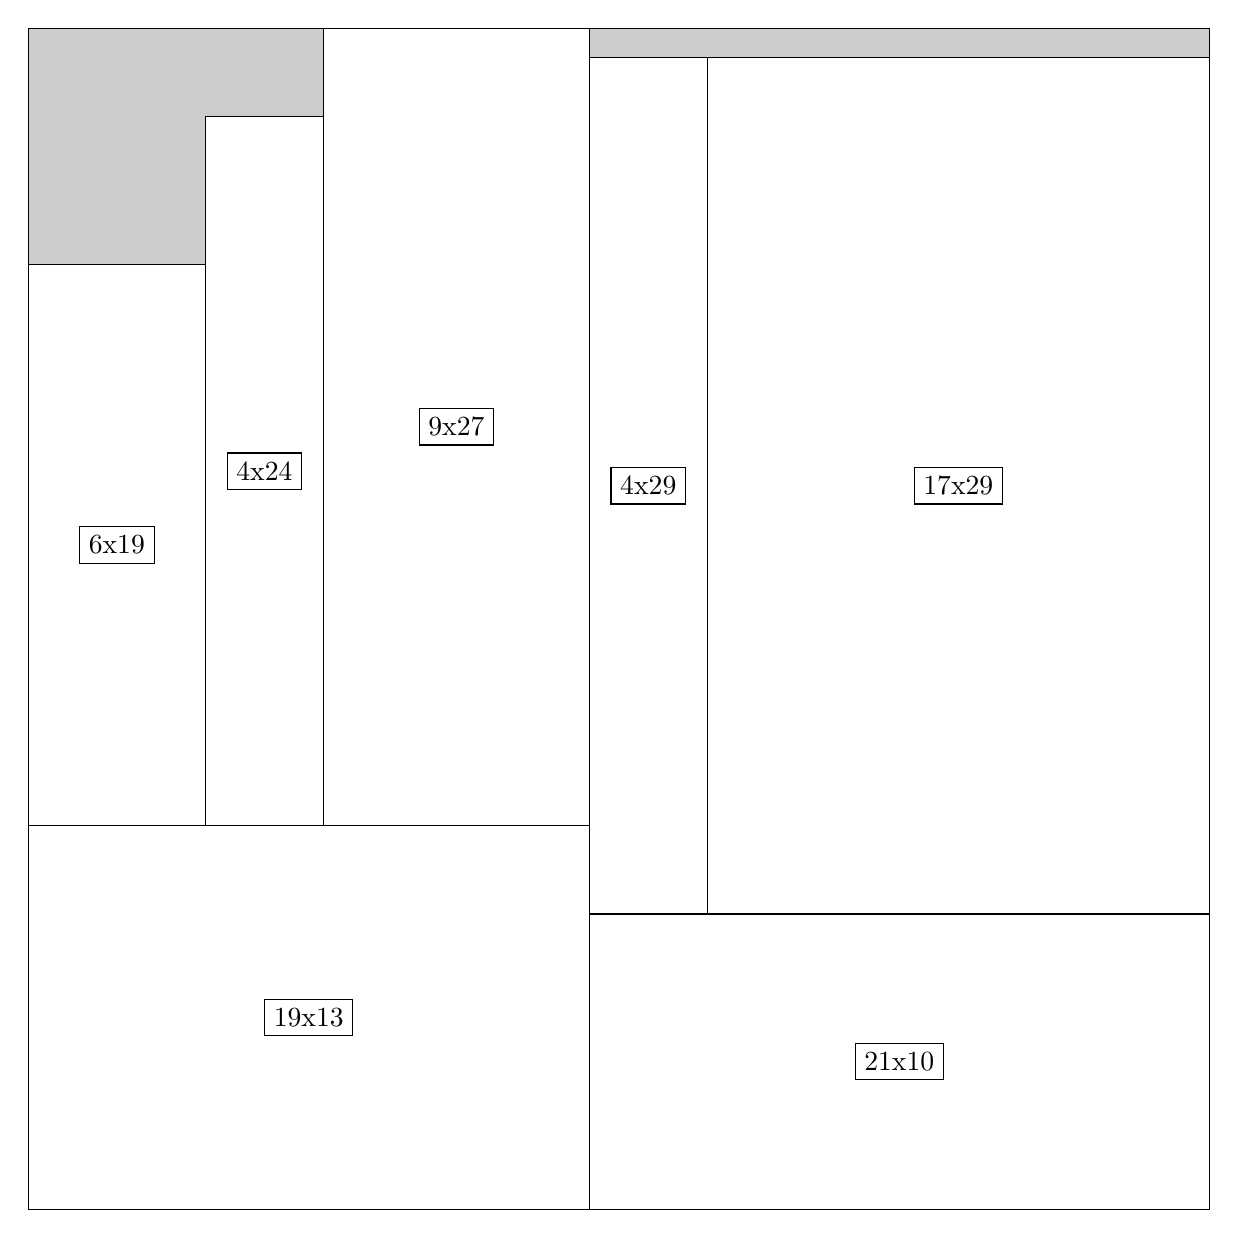
\begin{tikzpicture}[shorten >=1pt,scale=1.0,every node/.style={scale=1.0},->]
\tikzstyle{vertex}=[circle,fill=black!25,minimum size=14pt,inner sep=0pt]
\filldraw[fill=gray!40!white, draw=black] (0,0) rectangle (15.0,15.0);
\foreach \name/\x/\y/\w/\h in {21x10/7.125/0.0/7.875/3.75,17x29/8.625/3.75/6.375/10.875,4x29/7.125/3.75/1.5/10.875,19x13/0.0/0.0/7.125/4.875,9x27/3.75/4.875/3.375/10.125,4x24/2.25/4.875/1.5/9.0,6x19/0.0/4.875/2.25/7.125}
\filldraw[fill=white!40!white, draw=black] (\x,\y) rectangle node[draw] (\name) {\name} ++(\w,\h);
\end{tikzpicture}


w =21 , h =10 , x =19 , y =0 , v =210
\par
w =17 , h =29 , x =23 , y =10 , v =493
\par
w =4 , h =29 , x =19 , y =10 , v =116
\par
w =19 , h =13 , x =0 , y =0 , v =247
\par
w =9 , h =27 , x =10 , y =13 , v =243
\par
w =4 , h =24 , x =6 , y =13 , v =96
\par
w =6 , h =19 , x =0 , y =13 , v =114
\par
\newpage


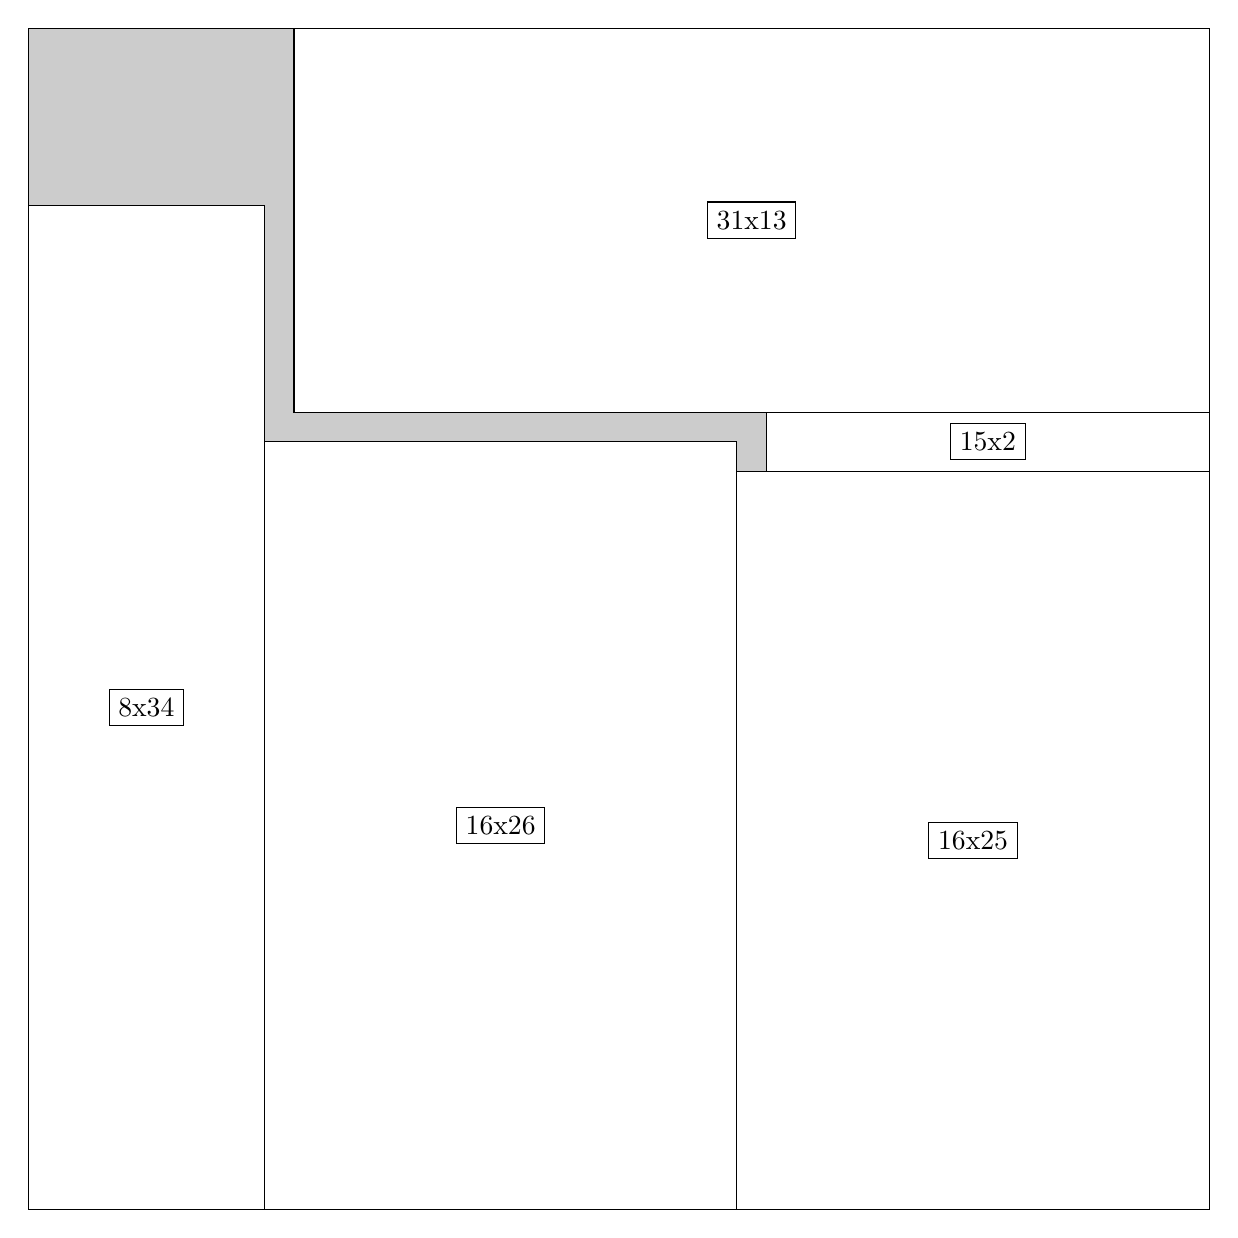
\begin{tikzpicture}[shorten >=1pt,scale=1.0,every node/.style={scale=1.0},->]
\tikzstyle{vertex}=[circle,fill=black!25,minimum size=14pt,inner sep=0pt]
\filldraw[fill=gray!40!white, draw=black] (0,0) rectangle (15.0,15.0);
\foreach \name/\x/\y/\w/\h in {16x25/9.0/0.0/6.0/9.375,15x2/9.375/9.375/5.625/0.75,16x26/3.0/0.0/6.0/9.75,31x13/3.375/10.125/11.625/4.875,8x34/0.0/0.0/3.0/12.75}
\filldraw[fill=white!40!white, draw=black] (\x,\y) rectangle node[draw] (\name) {\name} ++(\w,\h);
\end{tikzpicture}


w =16 , h =25 , x =24 , y =0 , v =400
\par
w =15 , h =2 , x =25 , y =25 , v =30
\par
w =16 , h =26 , x =8 , y =0 , v =416
\par
w =31 , h =13 , x =9 , y =27 , v =403
\par
w =8 , h =34 , x =0 , y =0 , v =272
\par
\newpage


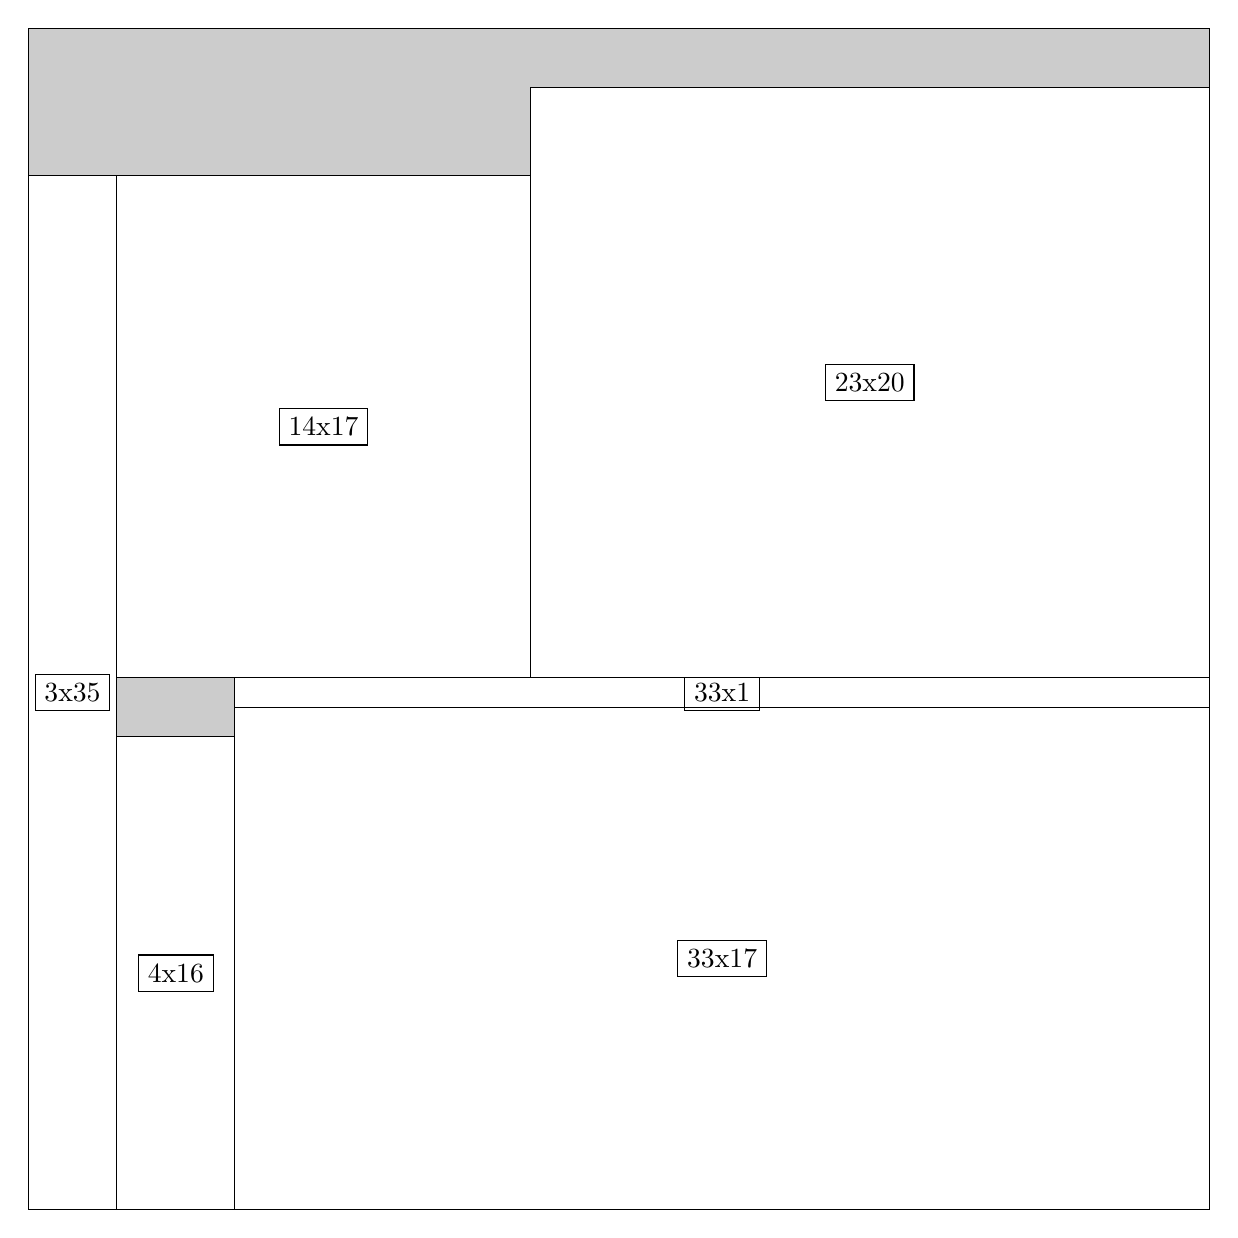
\begin{tikzpicture}[shorten >=1pt,scale=1.0,every node/.style={scale=1.0},->]
\tikzstyle{vertex}=[circle,fill=black!25,minimum size=14pt,inner sep=0pt]
\filldraw[fill=gray!40!white, draw=black] (0,0) rectangle (15.0,15.0);
\foreach \name/\x/\y/\w/\h in {33x17/2.625/0.0/12.375/6.375,4x16/1.125/0.0/1.5/6.0,33x1/2.625/6.375/12.375/0.375,23x20/6.375/6.75/8.625/7.5,14x17/1.125/6.75/5.25/6.375,3x35/0.0/0.0/1.125/13.125}
\filldraw[fill=white!40!white, draw=black] (\x,\y) rectangle node[draw] (\name) {\name} ++(\w,\h);
\end{tikzpicture}


w =33 , h =17 , x =7 , y =0 , v =561
\par
w =4 , h =16 , x =3 , y =0 , v =64
\par
w =33 , h =1 , x =7 , y =17 , v =33
\par
w =23 , h =20 , x =17 , y =18 , v =460
\par
w =14 , h =17 , x =3 , y =18 , v =238
\par
w =3 , h =35 , x =0 , y =0 , v =105
\par
\newpage


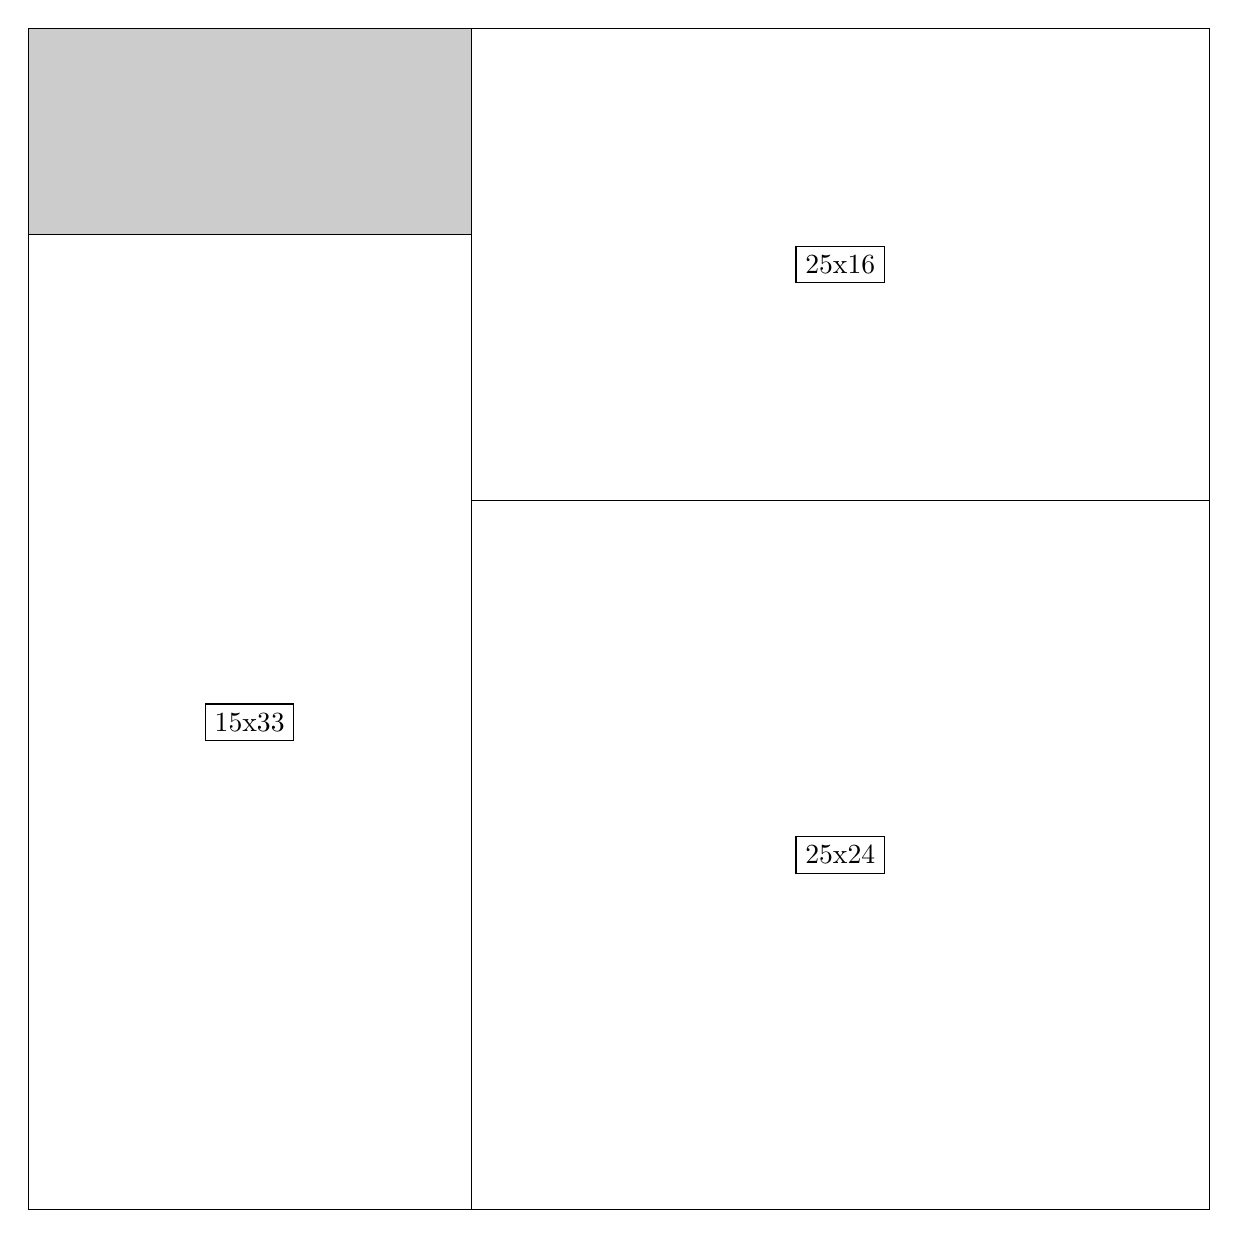
\begin{tikzpicture}[shorten >=1pt,scale=1.0,every node/.style={scale=1.0},->]
\tikzstyle{vertex}=[circle,fill=black!25,minimum size=14pt,inner sep=0pt]
\filldraw[fill=gray!40!white, draw=black] (0,0) rectangle (15.0,15.0);
\foreach \name/\x/\y/\w/\h in {25x24/5.625/0.0/9.375/9.0,25x16/5.625/9.0/9.375/6.0,15x33/0.0/0.0/5.625/12.375}
\filldraw[fill=white!40!white, draw=black] (\x,\y) rectangle node[draw] (\name) {\name} ++(\w,\h);
\end{tikzpicture}


w =25 , h =24 , x =15 , y =0 , v =600
\par
w =25 , h =16 , x =15 , y =24 , v =400
\par
w =15 , h =33 , x =0 , y =0 , v =495
\par
\newpage


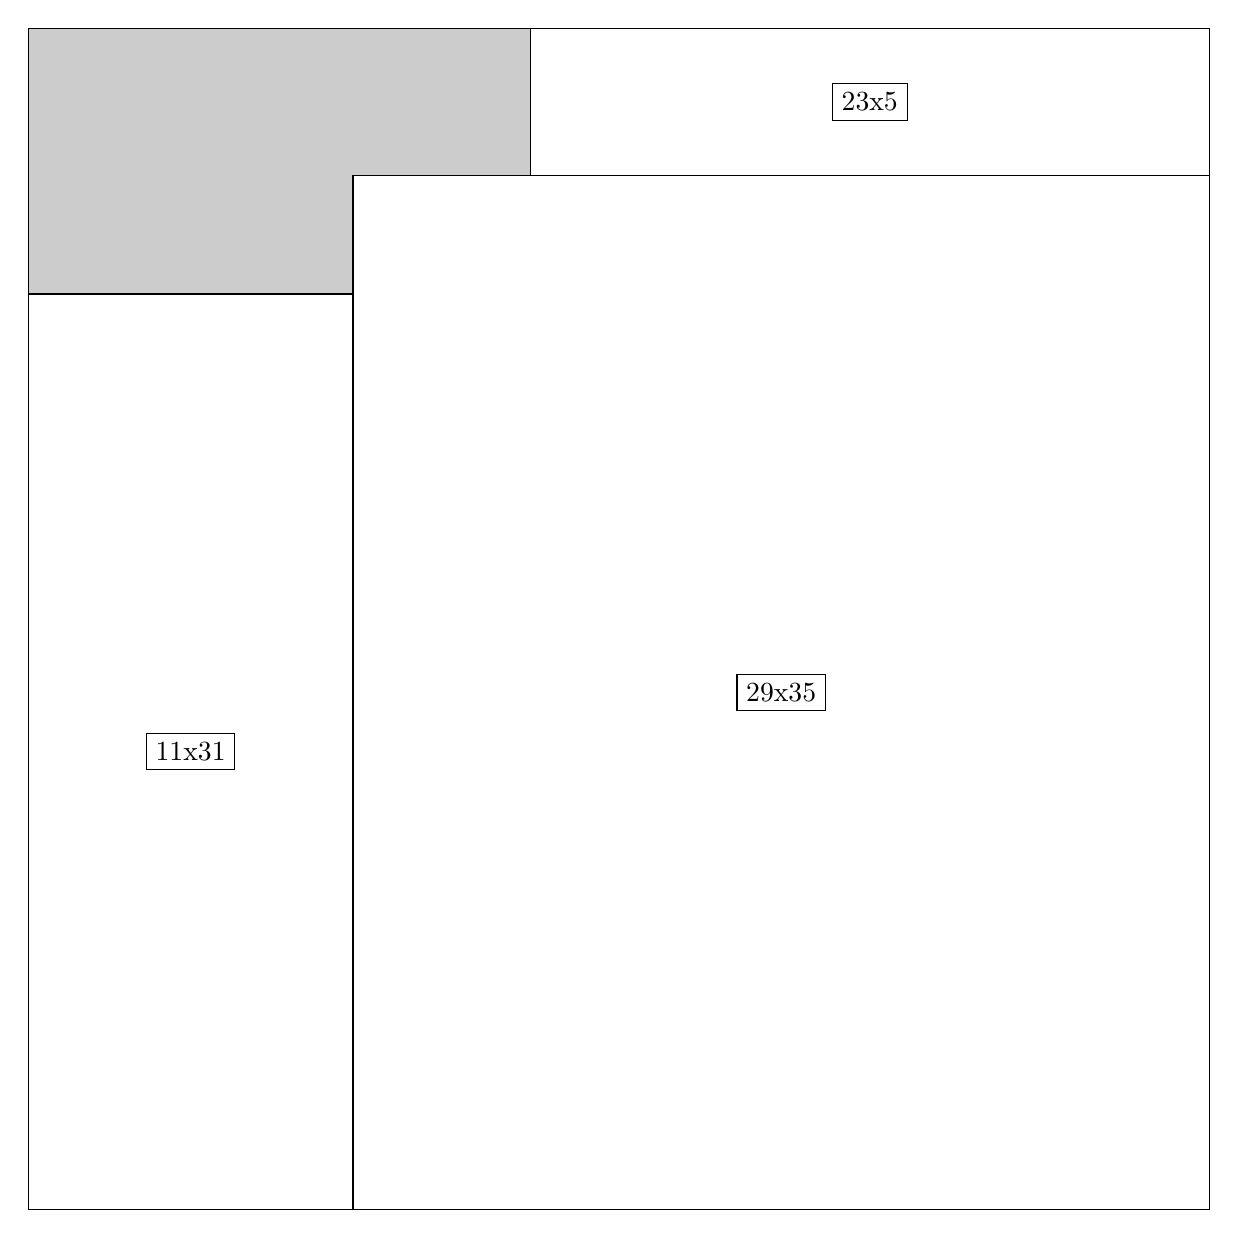
\begin{tikzpicture}[shorten >=1pt,scale=1.0,every node/.style={scale=1.0},->]
\tikzstyle{vertex}=[circle,fill=black!25,minimum size=14pt,inner sep=0pt]
\filldraw[fill=gray!40!white, draw=black] (0,0) rectangle (15.0,15.0);
\foreach \name/\x/\y/\w/\h in {29x35/4.125/0.0/10.875/13.125,11x31/0.0/0.0/4.125/11.625,23x5/6.375/13.125/8.625/1.875}
\filldraw[fill=white!40!white, draw=black] (\x,\y) rectangle node[draw] (\name) {\name} ++(\w,\h);
\end{tikzpicture}


w =29 , h =35 , x =11 , y =0 , v =1015
\par
w =11 , h =31 , x =0 , y =0 , v =341
\par
w =23 , h =5 , x =17 , y =35 , v =115
\par
\newpage


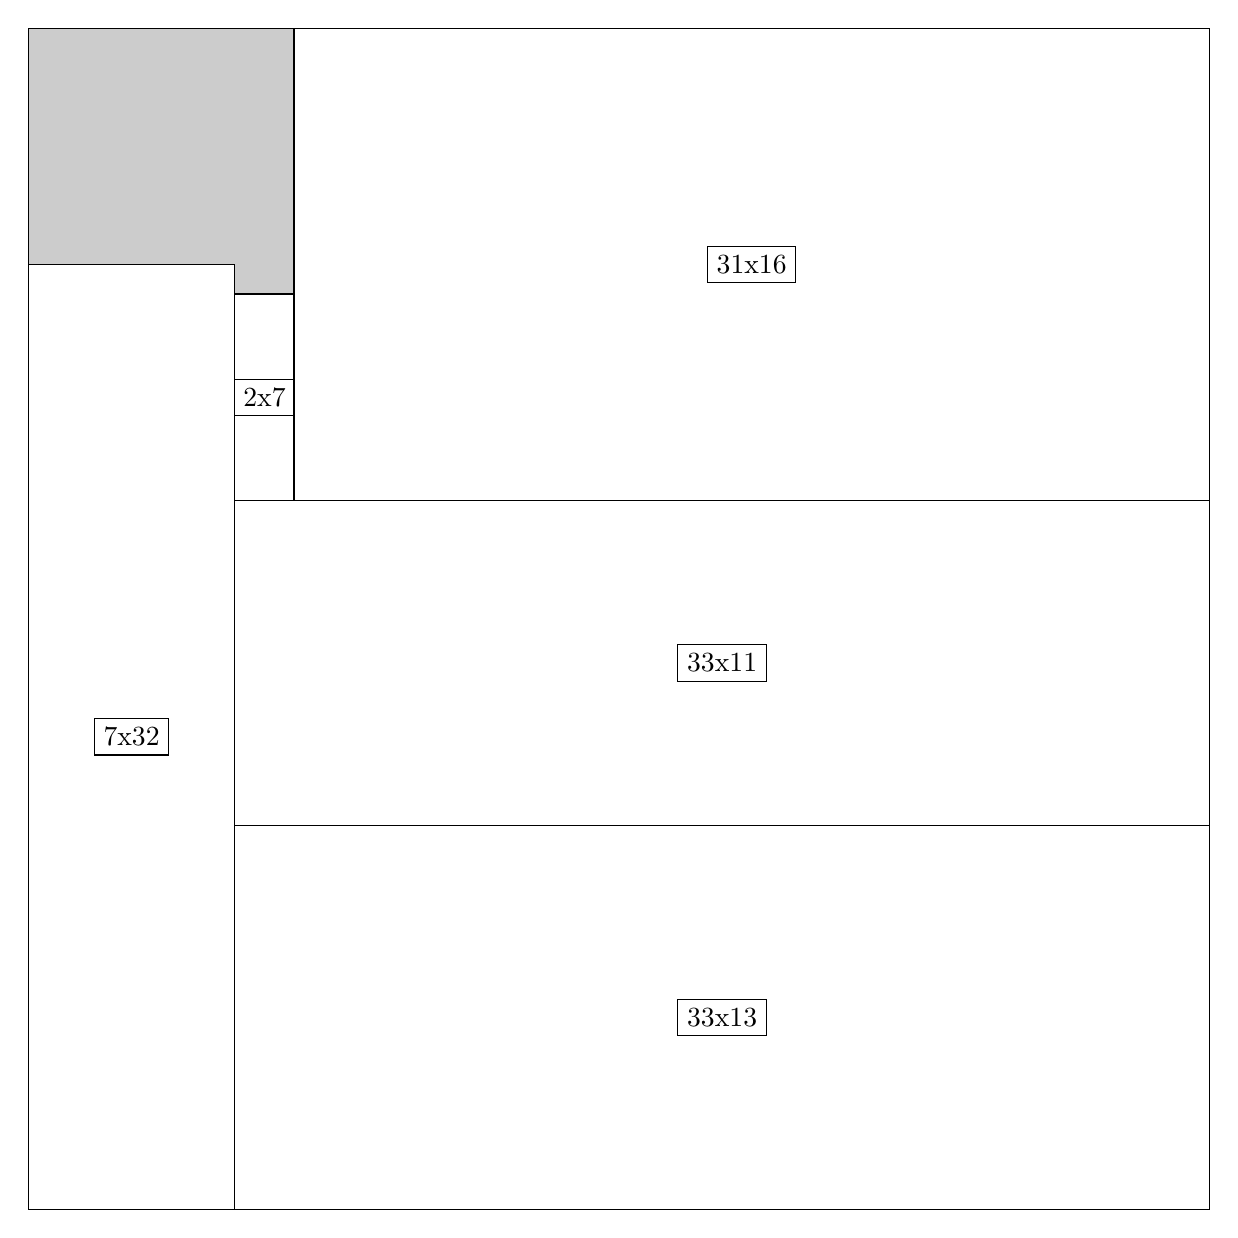
\begin{tikzpicture}[shorten >=1pt,scale=1.0,every node/.style={scale=1.0},->]
\tikzstyle{vertex}=[circle,fill=black!25,minimum size=14pt,inner sep=0pt]
\filldraw[fill=gray!40!white, draw=black] (0,0) rectangle (15.0,15.0);
\foreach \name/\x/\y/\w/\h in {33x13/2.625/0.0/12.375/4.875,33x11/2.625/4.875/12.375/4.125,31x16/3.375/9.0/11.625/6.0,2x7/2.625/9.0/0.75/2.625,7x32/0.0/0.0/2.625/12.0}
\filldraw[fill=white!40!white, draw=black] (\x,\y) rectangle node[draw] (\name) {\name} ++(\w,\h);
\end{tikzpicture}


w =33 , h =13 , x =7 , y =0 , v =429
\par
w =33 , h =11 , x =7 , y =13 , v =363
\par
w =31 , h =16 , x =9 , y =24 , v =496
\par
w =2 , h =7 , x =7 , y =24 , v =14
\par
w =7 , h =32 , x =0 , y =0 , v =224
\par
\newpage


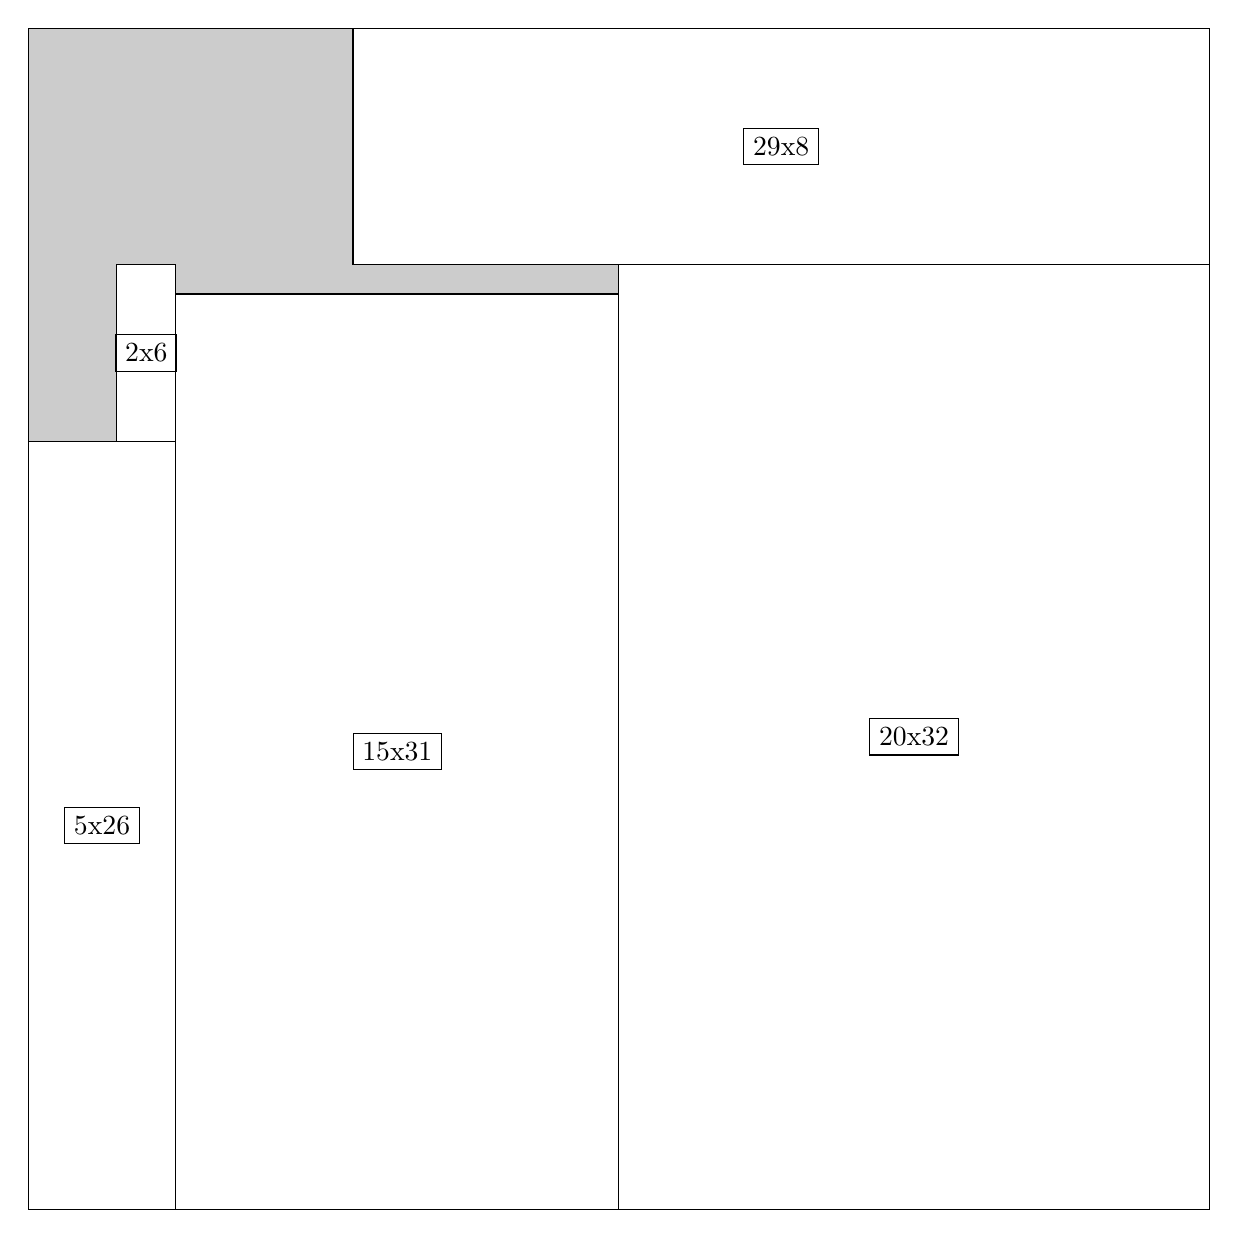
\begin{tikzpicture}[shorten >=1pt,scale=1.0,every node/.style={scale=1.0},->]
\tikzstyle{vertex}=[circle,fill=black!25,minimum size=14pt,inner sep=0pt]
\filldraw[fill=gray!40!white, draw=black] (0,0) rectangle (15.0,15.0);
\foreach \name/\x/\y/\w/\h in {20x32/7.5/0.0/7.5/12.0,15x31/1.875/0.0/5.625/11.625,5x26/0.0/0.0/1.875/9.75,2x6/1.125/9.75/0.75/2.25,29x8/4.125/12.0/10.875/3.0}
\filldraw[fill=white!40!white, draw=black] (\x,\y) rectangle node[draw] (\name) {\name} ++(\w,\h);
\end{tikzpicture}


w =20 , h =32 , x =20 , y =0 , v =640
\par
w =15 , h =31 , x =5 , y =0 , v =465
\par
w =5 , h =26 , x =0 , y =0 , v =130
\par
w =2 , h =6 , x =3 , y =26 , v =12
\par
w =29 , h =8 , x =11 , y =32 , v =232
\par
\newpage


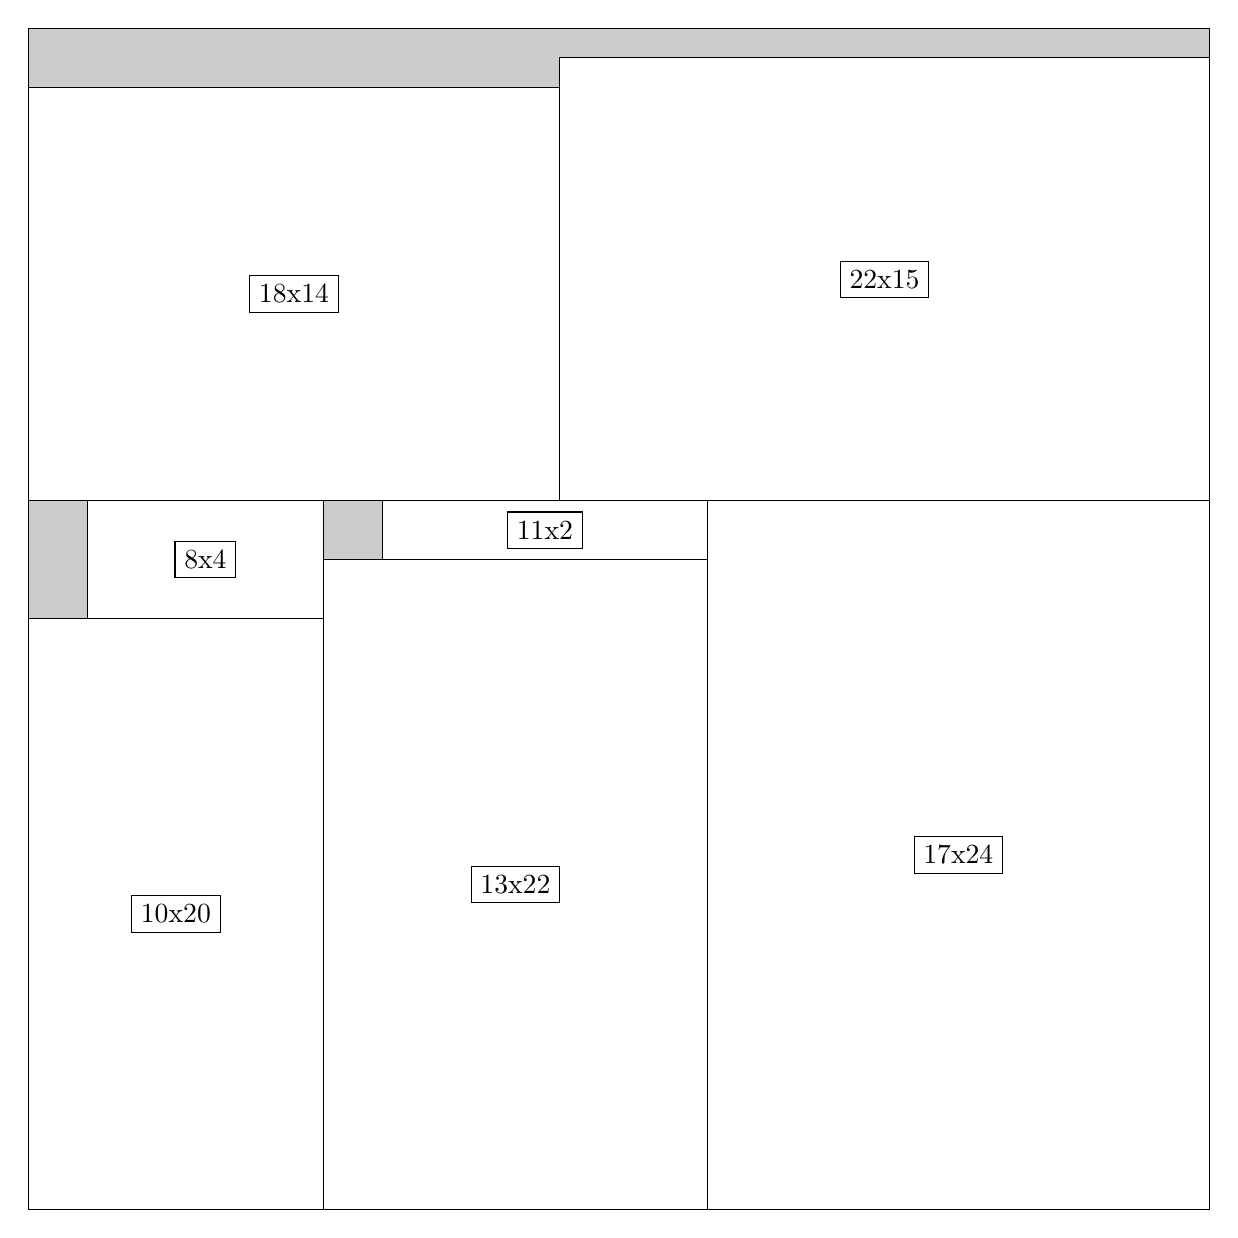
\begin{tikzpicture}[shorten >=1pt,scale=1.0,every node/.style={scale=1.0},->]
\tikzstyle{vertex}=[circle,fill=black!25,minimum size=14pt,inner sep=0pt]
\filldraw[fill=gray!40!white, draw=black] (0,0) rectangle (15.0,15.0);
\foreach \name/\x/\y/\w/\h in {17x24/8.625/0.0/6.375/9.0,13x22/3.75/0.0/4.875/8.25,11x2/4.5/8.25/4.125/0.75,10x20/0.0/0.0/3.75/7.5,8x4/0.75/7.5/3.0/1.5,22x15/6.75/9.0/8.25/5.625,18x14/0.0/9.0/6.75/5.25}
\filldraw[fill=white!40!white, draw=black] (\x,\y) rectangle node[draw] (\name) {\name} ++(\w,\h);
\end{tikzpicture}


w =17 , h =24 , x =23 , y =0 , v =408
\par
w =13 , h =22 , x =10 , y =0 , v =286
\par
w =11 , h =2 , x =12 , y =22 , v =22
\par
w =10 , h =20 , x =0 , y =0 , v =200
\par
w =8 , h =4 , x =2 , y =20 , v =32
\par
w =22 , h =15 , x =18 , y =24 , v =330
\par
w =18 , h =14 , x =0 , y =24 , v =252
\par
\newpage


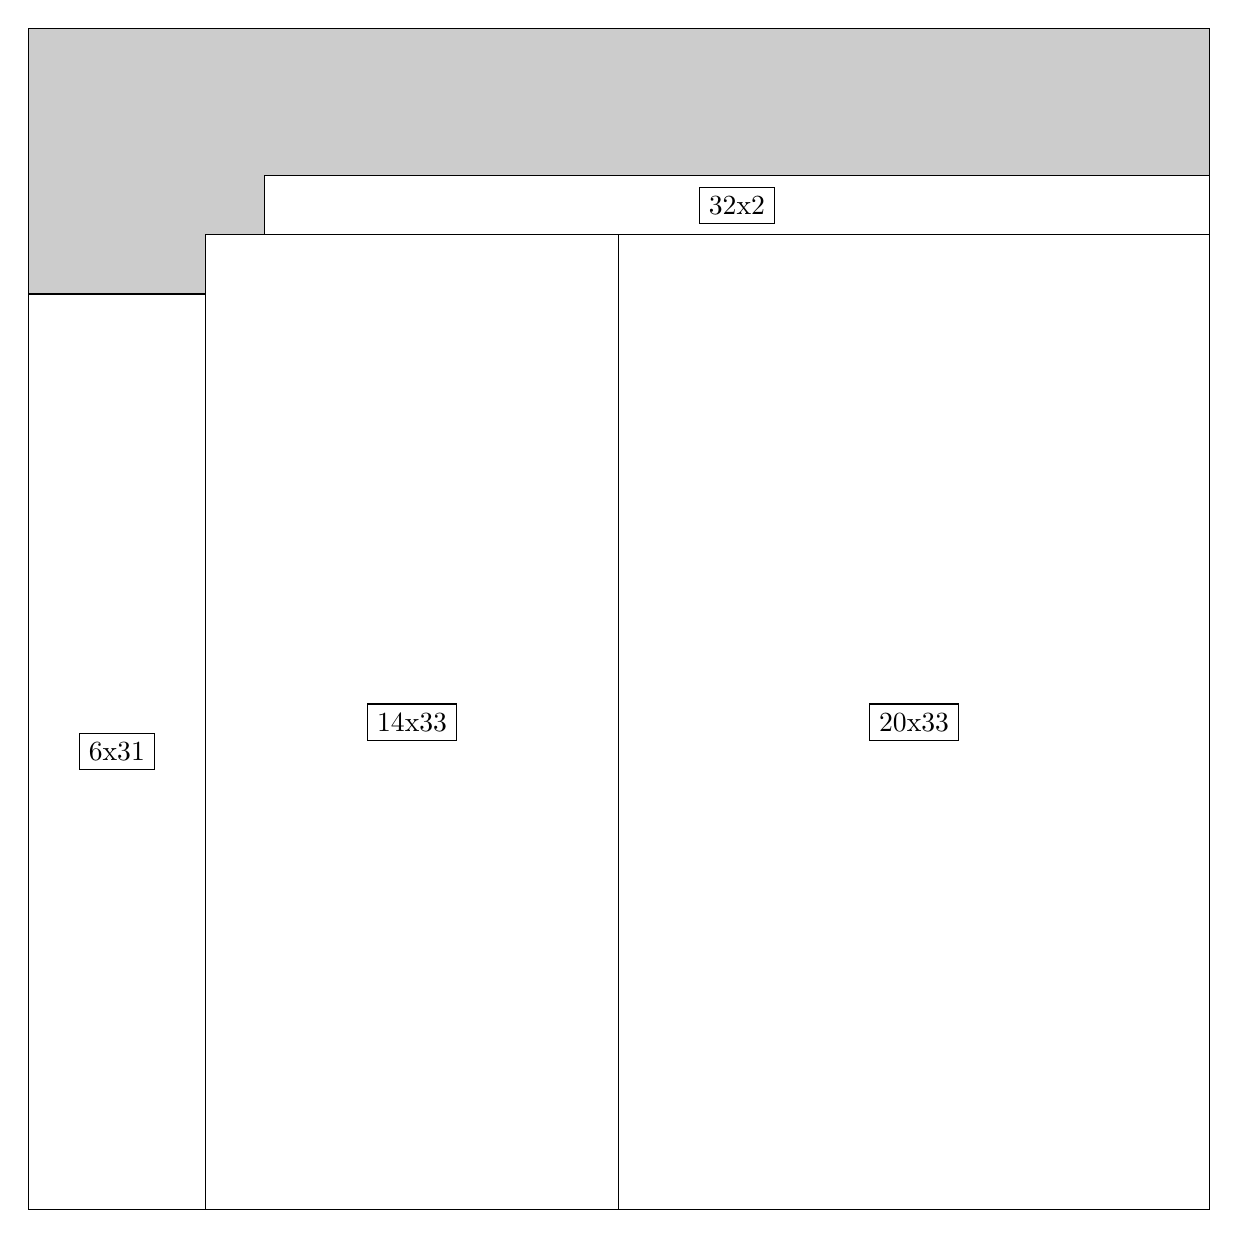
\begin{tikzpicture}[shorten >=1pt,scale=1.0,every node/.style={scale=1.0},->]
\tikzstyle{vertex}=[circle,fill=black!25,minimum size=14pt,inner sep=0pt]
\filldraw[fill=gray!40!white, draw=black] (0,0) rectangle (15.0,15.0);
\foreach \name/\x/\y/\w/\h in {20x33/7.5/0.0/7.5/12.375,14x33/2.25/0.0/5.25/12.375,6x31/0.0/0.0/2.25/11.625,32x2/3.0/12.375/12.0/0.75}
\filldraw[fill=white!40!white, draw=black] (\x,\y) rectangle node[draw] (\name) {\name} ++(\w,\h);
\end{tikzpicture}


w =20 , h =33 , x =20 , y =0 , v =660
\par
w =14 , h =33 , x =6 , y =0 , v =462
\par
w =6 , h =31 , x =0 , y =0 , v =186
\par
w =32 , h =2 , x =8 , y =33 , v =64
\par
\newpage


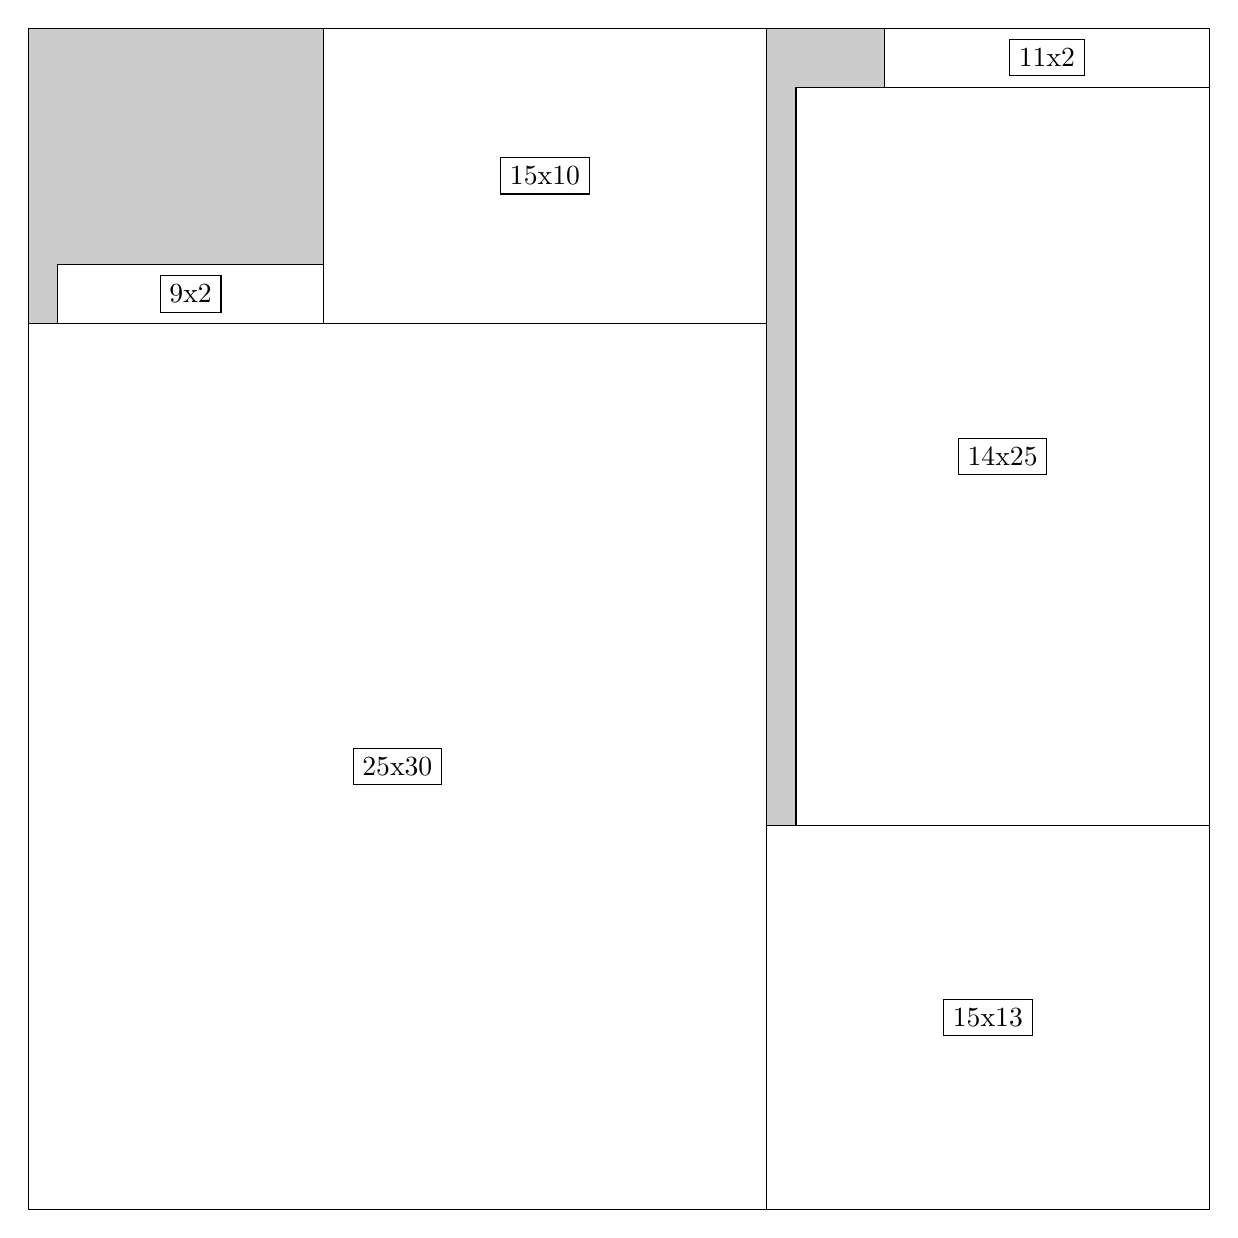
\begin{tikzpicture}[shorten >=1pt,scale=1.0,every node/.style={scale=1.0},->]
\tikzstyle{vertex}=[circle,fill=black!25,minimum size=14pt,inner sep=0pt]
\filldraw[fill=gray!40!white, draw=black] (0,0) rectangle (15.0,15.0);
\foreach \name/\x/\y/\w/\h in {15x13/9.375/0.0/5.625/4.875,14x25/9.75/4.875/5.25/9.375,11x2/10.875/14.25/4.125/0.75,25x30/0.0/0.0/9.375/11.25,15x10/3.75/11.25/5.625/3.75,9x2/0.375/11.25/3.375/0.75}
\filldraw[fill=white!40!white, draw=black] (\x,\y) rectangle node[draw] (\name) {\name} ++(\w,\h);
\end{tikzpicture}


w =15 , h =13 , x =25 , y =0 , v =195
\par
w =14 , h =25 , x =26 , y =13 , v =350
\par
w =11 , h =2 , x =29 , y =38 , v =22
\par
w =25 , h =30 , x =0 , y =0 , v =750
\par
w =15 , h =10 , x =10 , y =30 , v =150
\par
w =9 , h =2 , x =1 , y =30 , v =18
\par
\newpage


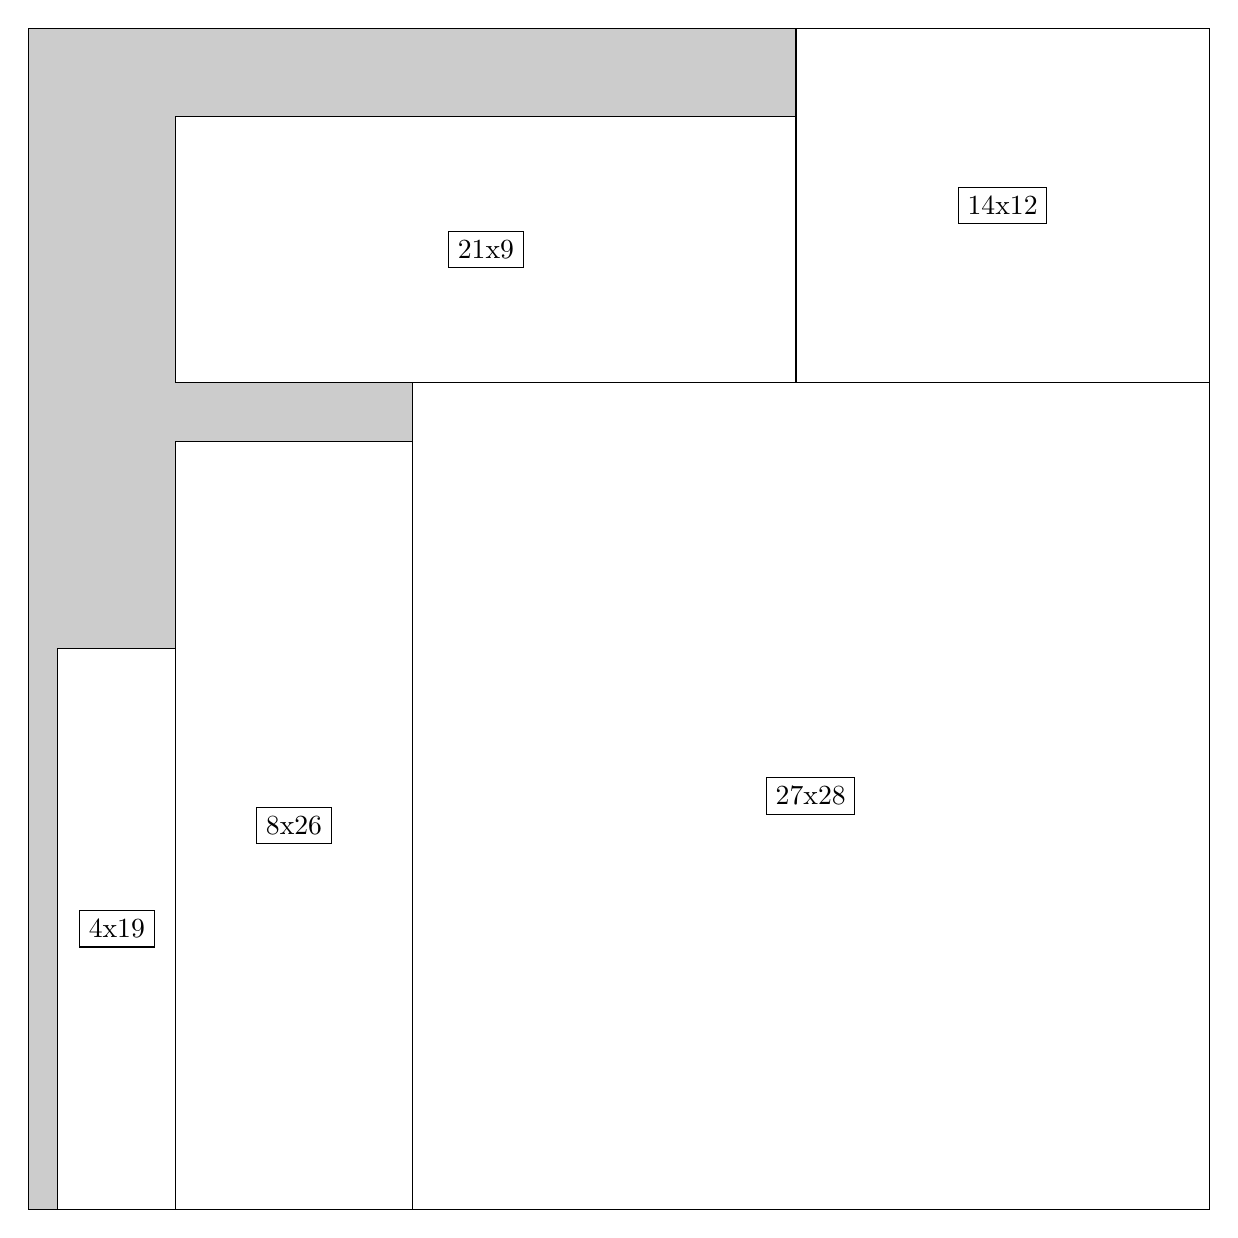
\begin{tikzpicture}[shorten >=1pt,scale=1.0,every node/.style={scale=1.0},->]
\tikzstyle{vertex}=[circle,fill=black!25,minimum size=14pt,inner sep=0pt]
\filldraw[fill=gray!40!white, draw=black] (0,0) rectangle (15.0,15.0);
\foreach \name/\x/\y/\w/\h in {27x28/4.875/0.0/10.125/10.5,8x26/1.875/0.0/3.0/9.75,4x19/0.375/0.0/1.5/7.125,14x12/9.75/10.5/5.25/4.5,21x9/1.875/10.5/7.875/3.375}
\filldraw[fill=white!40!white, draw=black] (\x,\y) rectangle node[draw] (\name) {\name} ++(\w,\h);
\end{tikzpicture}


w =27 , h =28 , x =13 , y =0 , v =756
\par
w =8 , h =26 , x =5 , y =0 , v =208
\par
w =4 , h =19 , x =1 , y =0 , v =76
\par
w =14 , h =12 , x =26 , y =28 , v =168
\par
w =21 , h =9 , x =5 , y =28 , v =189
\par
\newpage


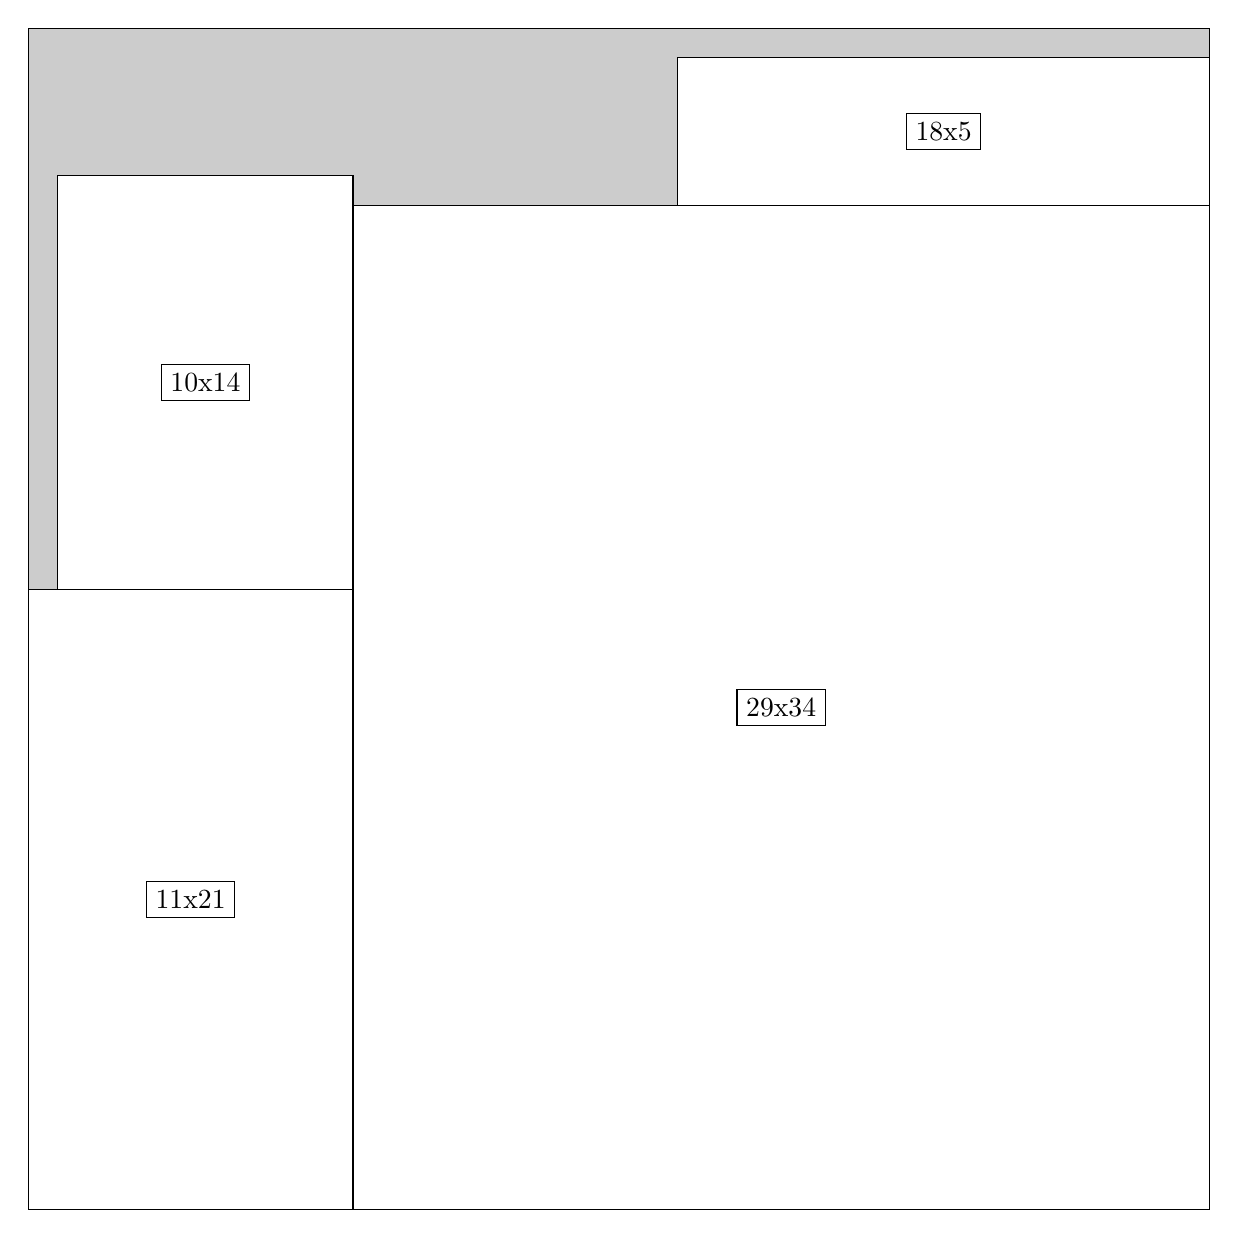
\begin{tikzpicture}[shorten >=1pt,scale=1.0,every node/.style={scale=1.0},->]
\tikzstyle{vertex}=[circle,fill=black!25,minimum size=14pt,inner sep=0pt]
\filldraw[fill=gray!40!white, draw=black] (0,0) rectangle (15.0,15.0);
\foreach \name/\x/\y/\w/\h in {29x34/4.125/0.0/10.875/12.75,18x5/8.25/12.75/6.75/1.875,11x21/0.0/0.0/4.125/7.875,10x14/0.375/7.875/3.75/5.25}
\filldraw[fill=white!40!white, draw=black] (\x,\y) rectangle node[draw] (\name) {\name} ++(\w,\h);
\end{tikzpicture}


w =29 , h =34 , x =11 , y =0 , v =986
\par
w =18 , h =5 , x =22 , y =34 , v =90
\par
w =11 , h =21 , x =0 , y =0 , v =231
\par
w =10 , h =14 , x =1 , y =21 , v =140
\par
\newpage


\end{document}